\begin{frame}{‌درخت جستجوی دودویی بهینه}
\begin{itemize}\itemr
\item[-]
فرض کنید می‌خواهیم برنامه‌ای طراحی کنیم که متون انگلیسی را به فارسی ترجمه کند. به ازای هر کلمهٔ انگلیسی در یک متن باید با استفاده از یک فرهنگ لغت، معادل فارسی آن را بیابیم. برای یک جستجوی بهینه می‌توانیم یک درخت جستجوی دودویی با n رأس بسازیم که هر رأس آن یک کلمهٔ انگلیسی و معادل فارسی آن را شامل شود.
\item[-]
اگر از یک درخت جستجوی دودویی متوازن
\fn{1}{balanced binary search tree}
%مانند درخت قرمز-سیاه
%\fn{2}{red-black tree}
استفاده کنیم، می‌توانیم جستجوی هر کلمه را در یک درخت با n کلمه در زمان
\m{O(\lg n)}
انجام دهیم.
\end{itemize}
\end{frame}

\begin{frame}{‌درخت جستجوی دودویی بهینه}
\begin{itemize}\itemr
\item[-]
اما کلمات مختلف تعداد تکرارهای مختلف دارند. برای مثال کلمات a یا the در انگلیسی بسیار پر تکرارند و بهتر است این کلمات در درخت جستجو به ریشه نزدیک‌تر باشند و برخی از اسامی خاص بسیار کم تکرارند و بهتر است که فاصلهٔ آنها از ریشه بیشتر باشد.
\item[-]
با استفاده از درخت جستجوی دودویی بهینه
\fn{1}{optimal binary search tree}
می‌توان کلمات را به گونه‌ای ذخیره و بازیابی کرد که کلمات با احتمال وقوع بیشتر نزدیک‌تر به ریشه قرار بگیرند.
\end{itemize}
\end{frame}


\begin{frame}{‌درخت جستجوی دودویی بهینه}
\begin{itemize}\itemr
\item[-]
دنبالهٔ
\m{K = \langle k_1, k_2, \cdots , k_n \rangle}
با n کلید را در نظر بگیرید به طوری‌که
\m{k_1 < k_2 < \cdots < k_n} .
\item[-]
می‌خواهیم یک درخت جستجوی دودویی بهینه حاوی این کلیدها بسازیم.
\item[-]
به ازای هر یک از کلیدهای
\m{k_i}
، یک احتمال وقوع
\m{p_i}
نیز داده شده است.
\item[-]
از آنجایی که برخی از کلیدها در درخت جستجو وجود ندارد‌ (برای مثال کلماتی در کاربرد ترجمه در انگلیسی وجود دارند که معادل فارسی ندارند) ، تعداد
\m{n+1}
کلید بی‌استفاده
\m{d_0, d_1, d_2, \cdots, d_n}
نیز داریم که نماینده این کلیدها هستند. در واقع
\m{d_0}
نمایندهٔ همهٔ کلیدهایی است که از
\m{k_1}
کوچکترند و
\m{d_n}
نمایندهٔ همهٔ کلیدهایی است که از
\m{k_n}
بزرگ‌ترند و همچنین به ازای
\m{i = 1,2, \cdots, n-1}
، کلید
\m{d_i}
نمایندهٔ همهٔ مقادیری است که بین
\m{k_i}
و
\m{k_{i+1}}
قرار دارند. همچنین به ازای هر کلید
\m{d_i}
یک احتمال وقوع
\m{q_i}
داریم.
\end{itemize}
\end{frame}


\begin{frame}{‌درخت جستجوی دودویی بهینه}
\begin{itemize}\itemr
\item[-]
در شکل زیر دو درخت جستجوی دودویی بهینه را با تعداد ۵ کلید مشاهده می‌کنیم.
\begin{figure}
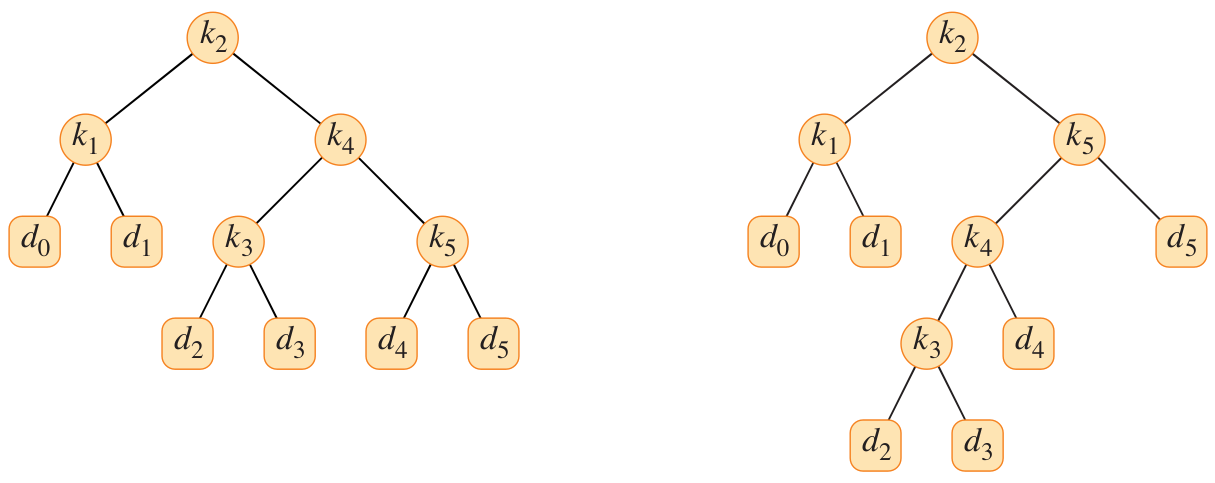
\includegraphics[width=0.9\textwidth]{figs/chap04/optimal-tree}
\end{figure}
\end{itemize}
\end{frame}


\begin{frame}{‌درخت جستجوی دودویی بهینه}
\begin{itemize}\itemr
\item[-]
هر یک از کلیدهای
\m{k_i}
یک رأس میانی است و هر یک از کلیدهای بی‌استفادهٔ
\m{d_i}
یک برگ در درخت جستجوی بهینه است.
\item[-]
از آنجایی که هر جستجو یا موفق است (که منجر به پیدا کردن یک کلید
\m{k_i}
می‌شود) و یا ناموفق (که منجر به رسیدن به کلید بی‌استفادهٔ
\m{d_i}
است)، بنابراین داریم :
\begin{align*}
\m{\sum_{i=1}^n p_i + \sum_{i=0}^n q_i = 1}
\end{align*}
\end{itemize}
\end{frame}


\begin{frame}{‌درخت جستجوی دودویی بهینه}
\begin{itemize}\itemr
\item[-]
با اطلاع داشتن از احتمال وقوع هر یک از کلید‌ها، می‌توانیم هزینه جستجو در یک درخت جستجو را پیدا کنیم.
\item[-]
فرض کنید هزینهٔ جستجوی یک کلید در درخت به ازای هر بار جستجو برابر با تعداد رئوس بررسی شده برای رسیدن به آن کلید باشد. بنابراین هزینهٔ جستجوی یک کلید در یک جستجو برابر خواهد بود با عمق
\fn{1}{depth}
رأس مربوط به آن کلید به علاوهٔ یک. ریشه در عمق صفر قرار دارد، بنابراین هزینهٔ یافتن کلید مربوط به ریشه در یک جستجو برابر است با یک.
\item[-]
برای یافتن هزینهٔ جستجوی یک کلید در یک متن، باید هزینهٔ یک بار جستجو را در احتمال وقوع آن کلید ضرب کنیم.
\item[-]
نهایتا برای یافتن هزینهٔ جستجوی یک درخت باید هزینهٔ جستجوی همهٔ کلیدها را با هم جمع کنیم.
\end{itemize}
\end{frame}

\newcommand{\depth}{\text{depth}}

\begin{frame}{‌درخت جستجوی دودویی بهینه}
\begin{itemize}\itemr
\item[-]
بنابراین هزینهٔ جستجو در درخت T برابر است با :
\begin{align*}
\m{E [\txtlr{search~cost~in}~T]} & \m{~= \sum_{i=1}^n (\depth_T (k_i)+1) \cdot p_i + \sum_{i=0}^n (\depth_T (d_i)+1) \cdot q_i}\\
& \m{~= 1 + \sum_{i=1}^n \depth_T (k_i) \cdot p_i + \sum_{i=0}^n \depth_T (d_i) \cdot q_i}
\end{align*}
\item[-]
در اینجا
\m{\depth_T}
تابعی است که عمق یک کلید را در درخت T نشان می‌دهد.
\end{itemize}
\end{frame}


\begin{frame}{‌درخت جستجوی دودویی بهینه}
\begin{itemize}\itemr
\item[-]
در شکل زیر هزینهٔ جستجو برای دو درخت جستجو محاسبه شده است.
\begin{figure}
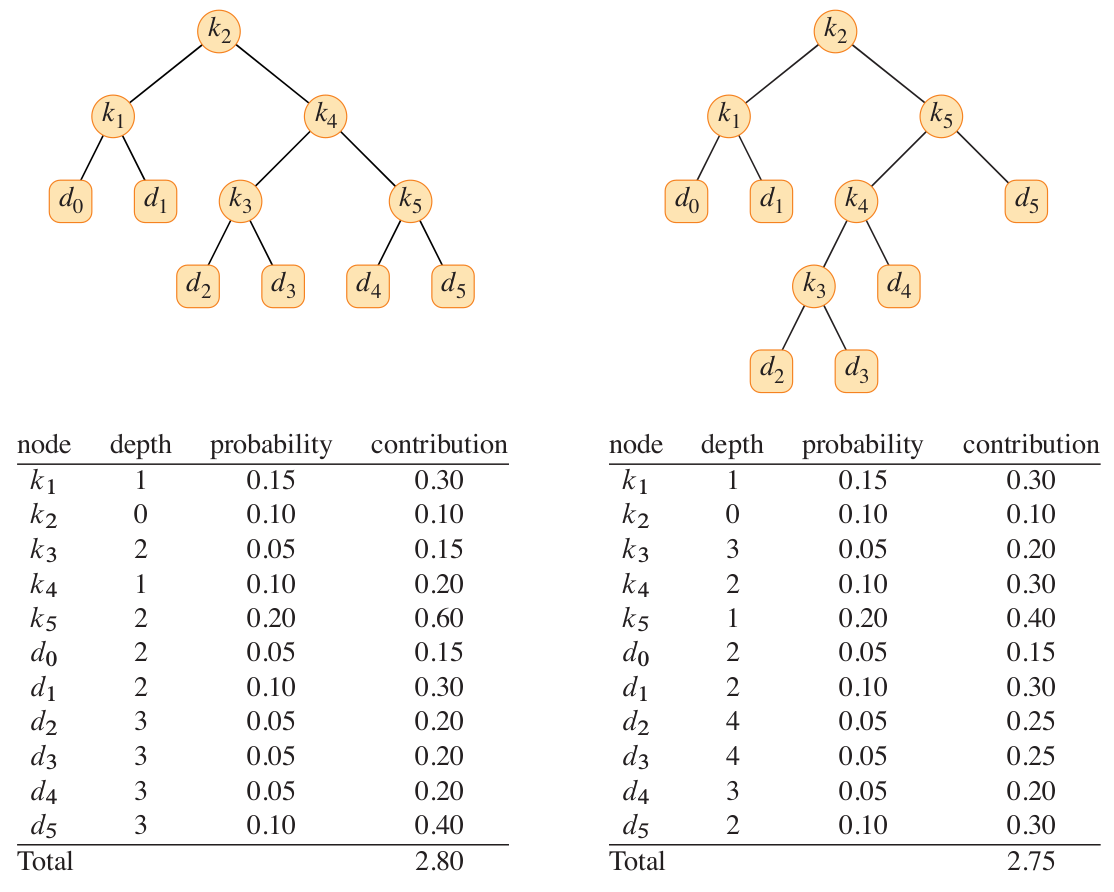
\includegraphics[width=0.6\textwidth]{figs/chap04/tree-cost}
\end{figure}
\end{itemize}
\end{frame}


\begin{frame}{‌درخت جستجوی دودویی بهینه}
\begin{itemize}\itemr
\item[-]
حال به ازای تعدادی کلید به همراه احتمال وقوع آنها، می‌خواهیم یک درخت جستجوی دودویی بیابیم که هزینهٔ جستجو در آن حداقل است.
\item[-]
به این درخت، درخت جستجوی دودویی بهینه
\fn{1}{optimal binary search tree}
گفته می‌شود.
\end{itemize}
\end{frame}


\begin{frame}{‌درخت جستجوی دودویی بهینه}
\begin{itemize}\itemr
\item[-]
در شکل زیر دو درخت جستجوی دودویی نشان داده شده‌اند. هزینهٔ جستجو در درخت سمت چپ
\m{2.80}
و در درخت سمت راست برابر با
\m{2.75}
است. درخت سمت راست یک درخت جستجوی بهینه است. در اینجا می‌توانیم ببینیم درخت جستجوی دودویی بهینه، الزاماً درختی نیست که عمق آن کمتر باشد.
\begin{figure}
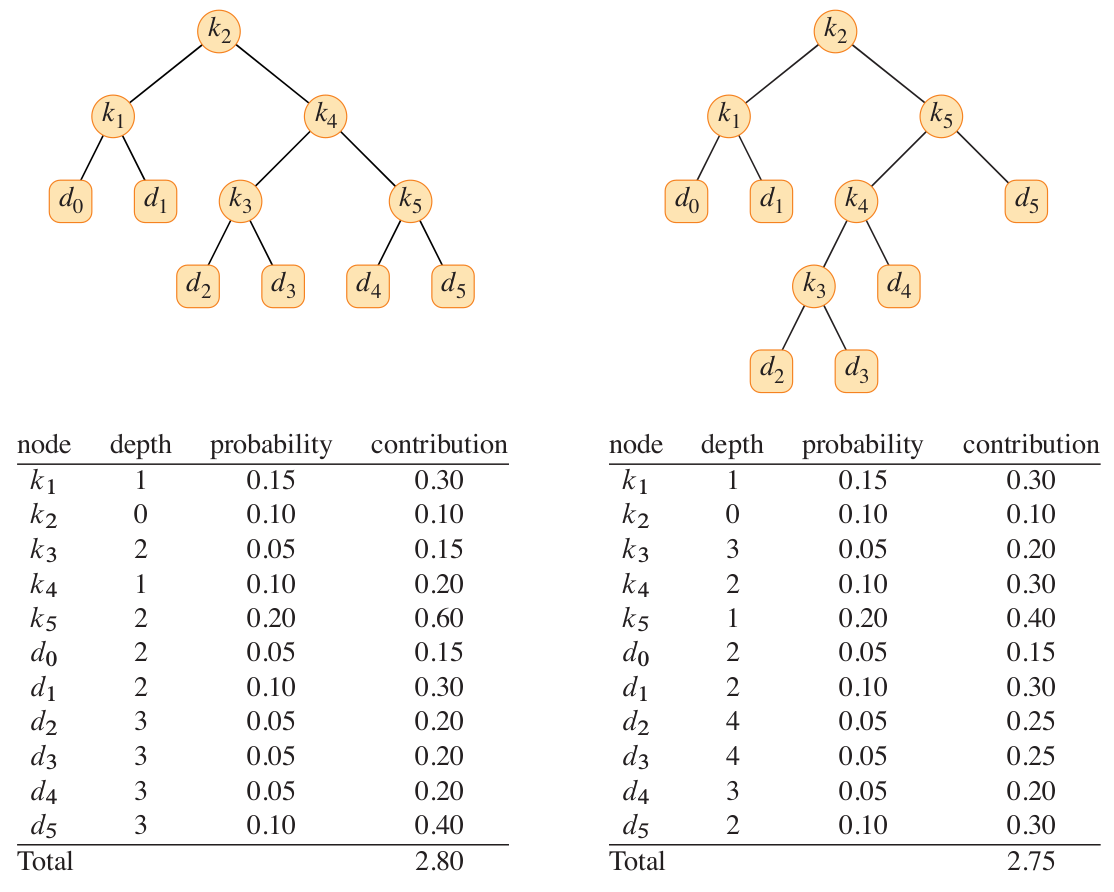
\includegraphics[width=0.5\textwidth]{figs/chap04/tree-cost}
\end{figure}
\end{itemize}
\end{frame}


\begin{frame}{‌درخت جستجوی دودویی بهینه}
\begin{itemize}\itemr
\item[-]
همچنین درخت جستجوی دودویی بهینه الزاماً درختی نیست که همهٔ کلیدها با احتمال وقوع بیشتر در ریشهٔ آن باشند. برای مثال کلید
\m{k_5}
بیشترین احتمال وقوع را دارد، اما ریشهٔ درخت جستجو
\m{k_2}
است.
\end{itemize}
\end{frame}


\begin{frame}{‌درخت جستجوی دودویی بهینه}
\begin{itemize}\itemr
\item[-]
همانند مسئله ضرب زنجیره‌ای ماتریس‌ها، با استفاده از جستجوی کامل برای بررسی همهٔ درخت‌های جستجو نمی‌توانیم در زمان چندجمله‌ای درخت جستجوی دودویی بهینه را به دست آوریم. تعداد همهٔ
 درخت‌های جستجوی دودویی از مرتبهٔ نمایی است، بنابراین بررسی همهٔ درخت‌های جستجو ممکن نیست.
\item[-]
می‌خواهیم این مسئله را با استفاده از برنامه‌ریزی پویا حل کنیم.
\end{itemize}
\end{frame}


\begin{frame}{‌درخت جستجوی دودویی بهینه}
\begin{itemize}\itemr
\item[-]
گام اول : ساختار یک درخت جستجوی دودویی بهینه
\item[-]
برای بررسی ساختار و مشخص کردن ویژگی‌های یک درخت بهینه، ابتدا ساختار درخت و زیردرخت‌های آن را بررسی می‌کنیم.
در واقع باید اثبات کنیم این مسئله دارای زیرساختار بهینه است، بدین معنی که جواب زیرمسئله‌ها را می‌توان از جواب مسئله استخراج کرد.
\item[-]
اگر یک درخت جستجوی دودویی بهینه
\m{T}
داشته باشیم، زیر درخت
\m{T'}
%شامل کلیدهای
%\m{k_i, \cdots, k_j}
%و کلیدهای
%\m{d_{i-1}, \cdots, d_j}
نیز باید بهینه باشد. اگر یک زیر درخت
\m{T''}
وجود داشت که هزینهٔ آن کمتر از
\m{T'}
بود، می‌توانستیم
\m{T'}
را با
\m{T''}
جایگزین کنیم و یک درخت با هزینه کمتر به جای
\m{T}
بیابیم که با فرض بهینه بودن
\m{T}
در تناقض است.
\item[-]
حال می‌خواهیم مسئله را با استفاده از جواب زیر مسئله‌های بهینهٔ آن حل کنیم.
\end{itemize}
\end{frame}


\begin{frame}{‌درخت جستجوی دودویی بهینه}
\begin{itemize}\itemr
\item[-]
یک زیردرخت دلخواه را در نظر بگیرید. این زیردرخت شامل کلیدهای
\m{k_i, \cdots, k_j}
است
که برگ‌های آن را کلیدهای
\m{d_{i-1}, \cdots, d_j}
تشکیل می‌دهند، به طوری‌که
\m{1 \leqslant i \leqslant j \leqslant n} .
\item[-]
به ازای کلیدهای
\m{k_i, \cdots, k_j}
، یکی از این کلیدها، برای مثال کلید
\m{k_r}
به طوری‌که
\m{i \leqslant r \leqslant j}
، ریشهٔ زیردرخت بهینه برای این کلیدهاست.
\item[-]
زیردرخت سمت چپ ریشهٔ
\m{k_r}
شامل کلیدهای
\m{k_i, \cdots, k_{r-1}}
و کلیدهای برگ
\m{d_{i-1}, \cdots, d_{r-1}}
است و زیردرخت سمت راست شامل کلیدهای
\m{k_{r+1}, \cdots, k_j}
و کلیدهای برگ
\m{d_r, \cdots, d_j}
است.
\item[-]
فرض کنید در یک زیردرخت با کلیدهای
\m{k_i, \cdots, k_j}
، کلید
\m{k_i}
را به عنوان ریشه انتخاب کنیم. 
%بنابراین زیردرخت سمت چپ این زیردرخت هیچ رأسی را شامل نمی‌شود. اگر برگ‌ها را نیز در نظر بگیریم، 
زیردرخت سمت چپ این زیردرخت یک برگ با کلید
\m{d_{i-1}}
است.
\item[-]
به طور مشابه، اگر
\m{k_j}
را به عنوان ریشه در نظر بگیریم زیر درخت سمت راست این زیر درخت شامل یک برگ با کلید
\m{d_j}
است.
\end{itemize}
\end{frame}


\begin{frame}{‌درخت جستجوی دودویی بهینه}
\begin{itemize}\itemr
\item[-]
گام دوم : راه حل بازگشتی
\item[-]
حال برای تعریف راه ‌حل بهینه به صورت بازگشتی، زیر درختی شامل کلیدهای
\m{k_i, \cdots, k_j}
را در نظر بگیرید به طوری‌که
\m{i \geqslant 1}
،
\m{j \leqslant n}
و
\m{j \geqslant i-1}
. وقتی
\m{j = i - 1}
باشد، تنها کلید برگ
\m{d_{i-1}}
را خواهیم داشت.
\item[-]
فرض کنید
\m{e[i,j]}
هزینهٔ جستجوی یک درخت جستجوی بهینه با کلیدهای
\m{k_i, \cdots, k_j}
باشد. هدف محاسبهٔ هزینه جستجو برای همهٔ کلیدهاست که برابر با مقدار
\m{e[1,n]}
می‌باشد.
\item[-]
اگر
\m{j = i - 1}
باشد، آنگاه مسئله تنها شامل یک کلید
\m{d_{i-1}}
می‌شود. در اینصورت هزینهٔ جستجو برابراست با
\m{e[i,i-1] = q_{i-1}}.
\item[-]
وقتی
\m{j \geqslant i}
باشد، باید ریشهٔ
\m{k_r}
را از بین کلیدهای
\m{k_i, \cdots, k_j}
انتخاب کنیم و یک درخت جستجوی بهینه با کلیدهای
\m{k_i, \cdots, k_{r-1}}
به عنوان زیردرخت سمت چپ ریشهٔ
\m{k_r}
و یک درخت جستجوی بهینه با کلیدهای
\m{k_{r+1}, \cdots, k_j}
به عنوان زیردرخت سمت راست ریشهٔ
\m{k_r}
بسازیم.
\end{itemize}
\end{frame}


\begin{frame}{‌درخت جستجوی دودویی بهینه}
\begin{itemize}\itemr
\item[-]
وقتی یک زیردرخت بهینه 
\m{T'}
 به عنوان زیردرخت یک رأس قرار می‌گیرد و درخت
\m{T}
را تشکیل می‌دهد،
 درواقع عمق هر یک از رأس‌های 
\m{T'}
در درخت
\m{T}
  یک واحد افزوده می‌شود. در اینصورت هزینهٔ جستجو برای رئوس زیردرخت
\m{T'}
در درخت
\m{T}
   به میزان مجموع احتمال رئوس 
\m{T'}
    افزایش می‌یابد.
\end{itemize}
\end{frame}

\begin{frame}{‌درخت جستجوی دودویی بهینه}
\begin{itemize}\itemr
\item[-]
برای مثال فرض کنید درخت
\m{T'}
 با کلید‌های
\m{k_1,k_2,k_3}
را تشکیل داده باشیم. هزینه جستجوی این درخت (بدون در نظر گرفتن کلیدهای بی‌استفاده) برابر است با
\m{E[T'] = \sum_{i=1}^3 (\depth_{T'}(k_i)+1) \cdot p_{i}  } .
\item[-]
اگر زیردرخت 
\m{T'}
در درخت 
\m{T}
قرار بگیرد به طوری که ریشه درخت 
\m{T}
کلید
\m{k_4}
و
\m{T'}
زیردرخت سمت چپ در درخت 
\m{T}
باشد، آنگاه خواهیم داشت:
\begin{align*}
\m{E[T]} =& \m{~p_4 + \Big(\sum_{i=1}^3 (\depth_{T}(k_i)+1 ) \cdot p_{i} \Big)} \\
=& \m{~p_4 + \Big( \sum_{i=1}^3 (\depth_{T'}(k_i)+2) \cdot p_{i} \Big) } \\
=& \m{~p_4 + E[T'] + \Big( \sum_{i=1}^3 p_{i} \Big) }
\end{align*}
\end{itemize}
\end{frame}

\begin{frame}{‌درخت جستجوی دودویی بهینه}
\begin{itemize}\itemr
\item[-]
برای یک زیردرخت با کلیدهای
\m{k_i, \cdots, k_j}
مجموع  احتمال‌ها برابر است با :
\begin{align*}
\m{w(i,j) = \sum_{l=i}^j p_l + \sum_{l=i-1}^j q_l}
\end{align*}
\item[-]
بنابراین اگر
\m{k_r}
ریشهٔ یک زیردرخت بهینه با کلیدهای
\m{k_i, \cdots, k_j}
باشد، خواهیم داشت :
\begin{align*}
\m{e[i,j] = p_r + (e[i,r-1] + w(i,r-1)) + (e[r+1,j] + w(r+1,j))}
\end{align*}
\end{itemize}
\end{frame}

\begin{frame}{‌درخت جستجوی دودویی بهینه}
\begin{itemize}\itemr
\item[-]
 از آنجایی که مجموع احتمال وقوع همهٔ رئوس در یک درخت برابر است با مجموع احتمال‌های وقوع رئوس زیردرخت چپ به علاوهٔ احتمال وقوع ریشه به علاوهٔ احتمال‌های وقوع رئوس زیردرخت راست، بنابراین رابطه زیر برقرار است :
\begin{align*}
\m{w(i,j) = w(i,r-1) + p_r + w(r+1,j)}
\end{align*}
\item[-]
بنابراین می‌توانیم رابطه بازگشتی برای محاسبه هزینهٔ جستجو در درخت بهینه را به صورت زیر بازنویسی کنیم :
\begin{align*}
\m{e[i,j] = e[i,r-1] + e[r+1,j] + w(i,j)}
\end{align*}
\end{itemize}
\end{frame}


\begin{frame}{‌درخت جستجوی دودویی بهینه}
\begin{itemize}\itemr
\item[-]
در اینجا فرض کردیم که می‌دانیم کدام رأس به عنوان رأس ریشهٔ
\m{k_r}
انتخاب می‌شود.
\item[-]
از آنجایی که هدف این است که ریشه‌ای را انتخاب کنیم که مقدار هزینه جستجو را کاهش دهد، بنابراین رابطهٔ بازگشتی برای محاسبهٔ هزینه جستجو در درخت بهینه را به صورت زیر می‌نویسیم.
\begin{align*}
\m{e[i,j]} = \left\{ \begin{array}{lr}
					\m{q_{i-1}} & \m{j=i-1}~~\text{اگر}\\
					\m{\min\{e[i,r-1] + e[r+1,j] + w(i,j) : i \leqslant r \leqslant j \}} & \m{i \leqslant j}~~ \text{اگر}
					\end{array}\right.
\end{align*}
\item[-]
بنابراین رابطه‌ای برای جدول
\m{e[i,j]}
جهت استفاده در یک الگوریتم برنامه‌ریزی پویا به صورت بازگشتی محاسبه کردیم.
\end{itemize}
\end{frame}


\begin{frame}{‌درخت جستجوی دودویی بهینه}
\begin{itemize}\itemr
\item[-]
جدول
\m{e[i,j]}
 تنها میزان هزینه جستجوی بهینه را نگهداری می‌کند.
\item[-]
 به یک جدول دیگر نیاز داریم برای اینکه بتوانیم ساختار درخت را نیز نگهداری کنیم تا در نهایت بتوانیم درخت جستجو بهینه را بازسازی کنیم.
\item[-]
این اطلاعات را در جدول
\m{root[i,j]}
نگهداری می‌کنیم. درواقع مقدار
\m{root[i,j]}
به ازای
\m{1 \leqslant i \leqslant j \leqslant n}
برابراست با اندیس r برای کلید
\m{k_r}
که ریشهٔ درخت جستجوی بهینه‌ای است که برای کلیدهای
\m{k_i, \cdots, k_j}
یافته می‌شود.
\end{itemize}
\end{frame}


\begin{frame}{‌درخت جستجوی دودویی بهینه}
\begin{itemize}\itemr
\item[-]
گام سوم : محاسبهٔ هزینهٔ جستجو در یک درخت جستجوی دودویی بهینه
\item[-]
حال با استفاده از روش برنامه‌ریزی پویا می‌توانیم مقادیر
\m{e[i,j]}
را به ترتیب از پایین به بالا محاسبه می‌کنیم. بنابراین کل جدول را به ازای
\m{e[1:n+1,0:n]}
مقداردهی می‌کنیم.
\item[-]
اندیس اول از 
\m{1}
 شروع شده و با
\m{n+1}
خاتمه می‌یابد، زیرا برای داشتن یک زیردرخت شامل تنها کلید
\m{d_n}
نیاز داریم
\m{e[n+1,n]}
را محاسبه کنیم. اندیس دوم باید از صفر شروع شود، زیرا برای داشتن یک زیردرخت تنها با کلید
\m{d_0}
، باید مقدار
\m{e[1,0]}
را محاسبه کنیم.
\item[-]
همهٔ مقادیر
\m{e[i,j]}
به ازای
\m{j \geqslant i-1}
باید محاسبه شوند. جدول
\m{root[i,j]}
ریشهٔ زیردرخت‌ها را با کلیدهای
\m{k_i, \cdots, k_j}
ذخیره می‌کند، به طوری‌که
\m{1 \leqslant i \leqslant j \leqslant n}.
\end{itemize}
\end{frame}


\begin{frame}{‌درخت جستجوی دودویی بهینه}
\begin{itemize}\itemr
\item[-]
همچنین می‌توانیم از یک جدول دیگر بهره بگیریم تا محاسبات را سریع‌تر انجام دهیم.
\item[-]
به جای محاسبه
\m{w(i,j)}
برای هر یک از درایه‌های
\m{e[i,j]}
%که به زمان
%\ath{j-i}
%نیاز دارد، 
جدول
\m{w[1:n+1,0:n]}
را محاسبه می‌کنیم. در حالت پایه، مقدار
\m{w[i,i-1] = q_{i-1}}
به ازای
\m{1 \leqslant i \leqslant n+1}
\item[-]
به ازای
\m{j \geqslant i}
درایه‌های جدول w را به صورت زیر محاسبه می‌کنیم.
\begin{align*}
\m{w[i,j] = w[i,j-1] + p_j + q_j}
\end{align*}
\item[-]
بنابراین می‌توانیم
\ath{n^2}
مقدار
\m{w[i,j]}
را هرکدام در زمان
\ath{1}
محاسبه کنیم.
% و مقادیر ذخیره شده در جدول را در زمان اجرا بازیابی کنیم.
\end{itemize}
\end{frame}


\begin{frame}{‌درخت جستجوی دودویی بهینه}
\begin{itemize}\itemr
\item[-]
الگوریتم زیر مسئلهٔ درخت جستجوی دودویی بهینه را به روش برنامه‌ریزی پویا حل می‌کند.
\begin{algorithm}[H]\alglr
  \caption{Optimal-BST} 
  \begin{algorithmic}[1]
   \Func{Optimal-BST}{p, q, n}
    \State let e[1:n+1 , 0:n], w[1:n+1 , 0:n], and root[1:n , 1:n] be new tables
    \For{i = 1 \To n + 1} \LeftComment{base cases} 
      \State e[i,i-1] = q[i-1]
      \State w[i,i-1] = q[i-1]
    \EndFor                        
  \end{algorithmic}
  \label{alg:merge}
\end{algorithm}
\end{itemize}
\end{frame}


\begin{frame}{‌درخت جستجوی دودویی بهینه}
\begin{itemize}\itemr
\item[-]
\begin{algorithm}[H]\alglr
  \caption{Optimal-BST} 
  \begin{algorithmic}[1]
  \setcounter{ALG@line}{4}
   \Func{Optimal-BST}{p, q, n}
    \For{t = 1 \To n}
    	\For{i = 1 \To n - t + 1}
    		\State j = i + t - 1
    		\State e[i,j] = $\infty$
    		\State w[i,j] = w[i,j-1] + p[j] + q[j]
    		 \For{r = i \To j} \LeftComment{try all possible roots r}
    		 		\State t = e[i,r-1] + e[r+1,j] + w[i,j] 
    		 		\If{t < e[i,j]} \LeftComment{new minimum?}
    		 				\State e[i,j] = t
    		 				\State root[i,j] = r
    		 		\EndIf
    		 \EndFor
    	\EndFor
    \EndFor
   \State \Return e and root                         
  \end{algorithmic}
  \label{alg:merge}
\end{algorithm}
\end{itemize}
\end{frame}


\begin{frame}{‌درخت جستجوی دودویی بهینه}
\begin{itemize}\itemr
\item[-]
الگوریتم درخت جستجوی دودویی بهینه محاسبات را در زمان
\ath{n^3}
انجام می‌دهد و به یک جدول با اندازهٔ
\ath{n^2}
نیاز دارد.
\end{itemize}
\end{frame}


\begin{frame}{‌درخت جستجوی دودویی بهینه}
\begin{itemize}\itemr
\item[-]
در شکل زیر، جدول‌های
\m{e[i,j]}
،
\m{w[i,j]}
و
\m{root[i,j]}
با استفاده از الگوریتم برنامه‌ریزی پویا برای جستجوی دودویی بهینه برای کلید‌های تعیین شده زیر، محاسبه شده‌اند.
\begin{figure}
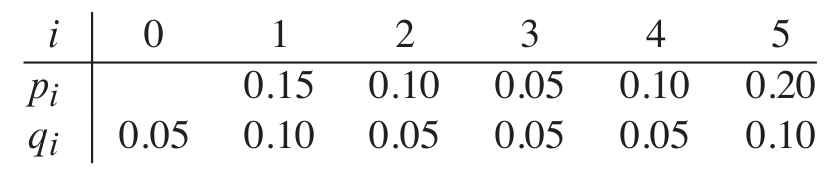
\includegraphics[width=0.5\textwidth]{figs/chap04/key-prob-example}
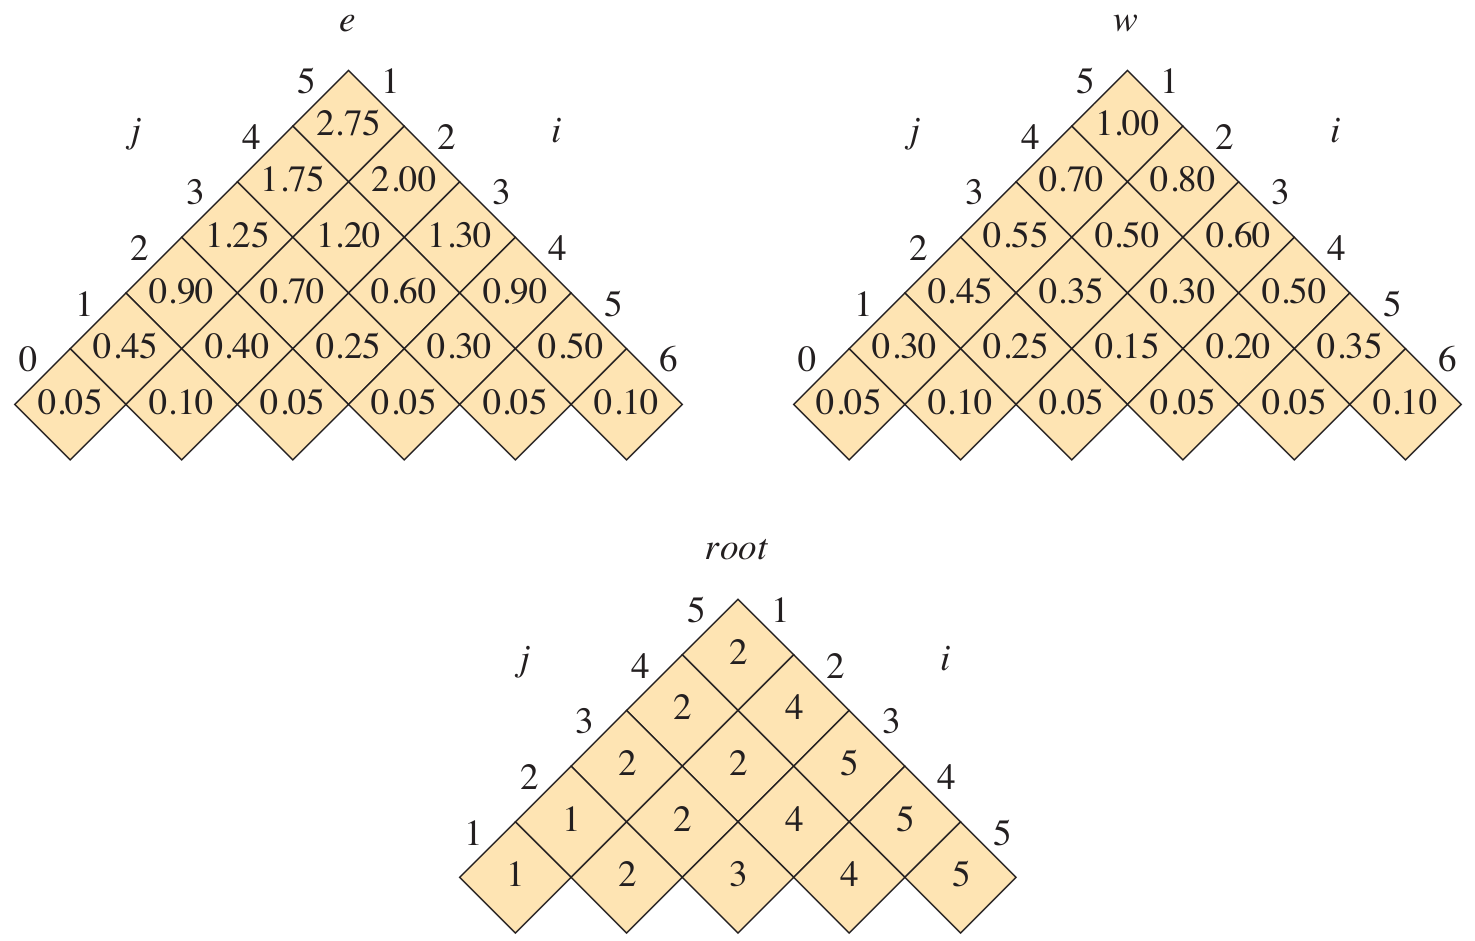
\includegraphics[width=0.5\textwidth]{figs/chap04/bst-example}
\end{figure}
\end{itemize}
\end{frame}